\documentclass[aspectratio=169, t, 8pt]{beamer}

%------configurando acentos-----------
\usepackage[utf8]{inputenc}
\usepackage[brazil]{babel}

\usepackage{graphicx}

%-------Estilos Beamer---------------
\usetheme{metropolis}
%\usecolortheme{crane}
%\usefonttheme{serif}
\linespread{1.2}

% Personalização de Cores (Exemplo: Minimal Teal)
% Cores Base
\definecolor{BgCanvas}{HTML}{F9F9FB}      % Off-white muito suave
\definecolor{MainText}{HTML}{2B2D42}      % Grafite escuro para alta legibilidade
\definecolor{PrimaryAccent}{HTML}{4A6FA5} % Az
\definecolor{SunCoastFg}{HTML}{F2A154}
% --- CONFIGURAÇÕES DE TEMA BEAMER ---
%\usetheme{metropolis}

\setbeamertemplate{itemize item}{\textcolor{MainText}{$\bullet$}}
\setbeamertemplate{itemize subitem}{\textcolor{MainText}{\scriptsize$\circ$}}
\setbeamertemplate{itemize 3rditem}{\textcolor{MainText}{\tiny$\blacksquare$}}

\setbeamercolor{background canvas}{bg=BgCanvas}
\setbeamercolor{normal text}{fg=MainText}
\setbeamercolor{frametitle}{bg=SunCoastFg, fg=BgCanvas}
\setbeamercolor{title}{fg=MainText}
\setbeamercolor{subtitle}{fg=PrimaryAccent}
\setbeamercolor{structure}{fg=PrimaryAccent}

% Remove a linha amarela padrão do Metropolis sob o título
\setbeamertemplate{title separator}{}
\setbeamertemplate{progress bar in section page}{}


%--------Dados do Documento
\title{Matemática: Lista de Exercícios}
\author{prof. Eduardo}
\institute{Pré-Universitário Oficina do Saber / UFF}
\date{\today}


%-------- Pacotes Matemática -------------
\usepackage{amsmath}
\usepackage{amsthm}
\usepackage{amsfonts}
\usepackage{amssymb}
\usepackage{xfrac}
\usepackage{thmtools}

%-------- Configuração Listas---------
\usepackage{enumitem}

\setcounter{tocdepth}{2}

\newcounter{questaovest}
\newcommand{\vest}[1]{\stepcounter{questaovest}\item[\textbf{Questão \arabic{questaovest}} (#1):]}
\setlist[enumerate]{
    align=left,
    leftmargin=1.8em,
    itemindent=1.8em
    }

\setlist[enumerate,2]{
    label=\alph*.,
    font=\bfseries,
    itemsep=0.1pt,
    labelsep=0em,
    parsep=0pt,
    leftmargin=0em
    }

%------------- Atalho para imagens ------------
\graphicspath{{./src/img/}}


\begin{document}

    \begin{frame}[plain]

        \vspace*{\fill}
        \begin{columns}[c]
            \begin{column}{0.5\textwidth}
                {\usebeamerfont{title}\usebeamercolor[fg]{title}\inserttitle}\vspace{0.2cm}
                    
                {\usebeamerfont{subtitle}\usebeamercolor[fg]{subtitle}\insertsubtitle}\vspace{0.5cm}

                {\usebeamerfont{author}\insertauthor}\vspace{0.3cm}

                {\usebeamerfont{institute}\insertinstitute}\vspace{0.3cm}

                {\usebeamerfont{date}\insertdate}
            \end{column}

            \begin{column}{0.4\textwidth}
                \centering
                
\includegraphics[width=0.4\textwidth]{logo_ofSaber.png}
            \end{column}
        \end{columns}
    \end{frame}

    \begin{frame}
        \frametitle{Geometria}
        \begin{enumerate}
            \begin{columns}
                \begin{column}{.9\textwidth}
                    \vest{IFBA-2018} Abaixo estão duas retas paralelas cortadas por duas transversais e um triângulo retângulo. Então, o valor da área de um quadrado de lado ''$y$'' u.c., em unidades de área, é?
                \end{column}
            \end{columns}

            
                \begin{columns}
                    \begin{column}{.3\textwidth}
                        \begin{figure}[H]
                            \centering
                        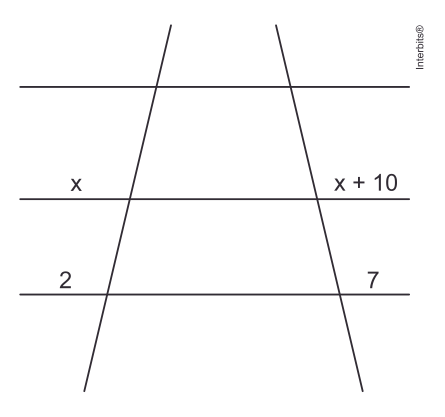
\includegraphics[width=\textwidth]{q01fig01.png}
                    \end{figure}
                \end{column}

                \begin{column}{.3\textwidth}
                    \begin{figure}[H]
                        \centering
                        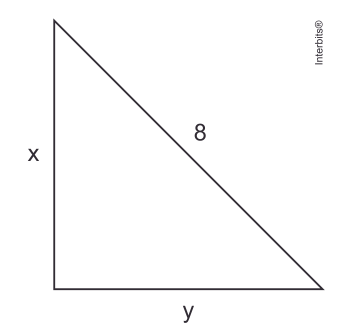
\includegraphics[width=\textwidth]{q01fig02.png}
                    \end{figure}
                \end{column}

                \begin{column}{.1\textwidth}
                    \begin{enumerate}
                        \item $48$
                        \item $58$
                        \item $32$
                        \item $16$
                        \item $28$
                        %gabarito: A
                    \end{enumerate}
                \end{column}
            \end{columns}
        \end{enumerate}
    
    \end{frame}

    \begin{frame}
        \frametitle{Geometria}
        \begin{columns}
            \begin{column}{0.9\textwidth}
                \begin{enumerate}
                    \vest{Cesgranrio-1996} Na Figura a seguir, $AB$ e $CD$ são paralelos. Se $AB=136$, $CE=75$ e $CD=50$. Quanto mede o segmento $AE$?
                    
                    \begin{columns}
                        \begin{column}{0.6\textwidth}
                            \begin{figure}[H]
                                \centering
                                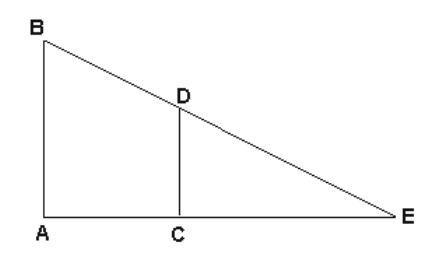
\includegraphics[width=.9\textwidth]{q02fig1.png}
                            \end{figure}
                        \end{column}

                        \begin{column}{.2\textwidth}
                            \begin{enumerate}
                                \item 136
                                \item 306
                                \item 204
                                \item 163
                                %gabarito: c
                    \end{enumerate}
                        \end{column}
                    \end{columns}
                \end{enumerate}
            \end{column}
        \end{columns}
    \end{frame}
   
    \begin{frame}
        \frametitle{Matemática Básica}
        \begin{columns}
            \begin{column}{.9\textwidth}
                \begin{enumerate}
            \vest{ESPM-2017} Uma senhora foi ao shopping e gastou a metade do dinheiro que tinha na carteira e pagou R\$ 10,00 de estacionamento. Ao voltar para casa parou numa livraria e comprou um livro que custou a quinta parte do que lhe havia sobrado, ficando com R\$ 88,00.

            Se ela tivesse ido apenas à livraria e comprado o mesmo livro, teria restado:
            \vspace{.2cm}
            \begin{enumerate}
                \item R\$ 218,00
                \item R\$ 186,00
                \item R\$ 154,00
                \item R\$ 230,00
                \item R\$ 120,00
            \end{enumerate}
        \end{enumerate}
            \end{column}
        \end{columns}
    \end{frame}

    \begin{frame}
        \frametitle{Progressão Aritmética}
        \begin{columns}
            \begin{column}{.9\textwidth}
                \begin{enumerate}
            \vest{ENEM-2ª apl-2010} A corrida de rua cresce no Brasil. Nunca se falou tanto no assunto como hoje, e a quantidade de adeptos aumenta progressivamente, afinal, correr traz inúmeros benefícios para a saúde física e mental, além de ser um esporte que não exige alto investimento financeiro.

            \vspace{0.2cm}
            
            Um corredor estipulou um plano de treinamento diário, correndo 3 quilômetros no primeiro dia e aumentando 500 metros por dia, a partir do segundo. Contudo, seu médico cardiologista autorizou essa atividade até que o corredor atingisse, no máximo, 10 km de corrida em um mesmo dia de treino. Se o atleta cumprir a recomendação médica e praticar o treinamento estipulado corretamente em dias consecutivos, pode-se afirmar que esse planejamento de treino só poderá ser executado em, exatamente,

            \vspace{0.2cm}

            \begin{enumerate}
                \item 12 dias
                \item 13 dias
                \item 14 dias
                \item 15 dias
                \item 16 dias
            \end{enumerate}
        \end{enumerate}
            \end{column}
        \end{columns}
    \end{frame}

    \begin{frame}
        \frametitle{Funções}
       \begin{columns}
            \begin{column}{.9\textwidth}
                 \begin{enumerate}
            \vest{PUCRJ-2013} Sejam $f$ e $g$ funções reais dadas por $f(x)=2+x^{2}$ e $g(x)=2+x$. Os valores de $x$ tais que $f(x)=g(x)$ são:

             \begin{enumerate}
                \item $x=0$ ou $x=-1$
                \item $x=0$ ou $x=2$
                \item $x=0$ ou $x=1$
                \item $x=2$ ou $x=-1$
                \item $x=0$ ou $x=1/2$
            \end{enumerate}
        \end{enumerate}
            \end{column}
       \end{columns}
    \end{frame}

    \begin{frame}
        \frametitle{Funções}
        \begin{columns}
            \begin{column}{0.9\textwidth}
                \begin{enumerate}
            \vest{ESPEcEx/AMAN-2013} Na figura abaixo está representado o gráfico de uma função real do 1º grau $f(x)$.

            \begin{columns}
                \begin{column}{0.5\textwidth}
                    \begin{figure}[!htbp]
                        \centering
                        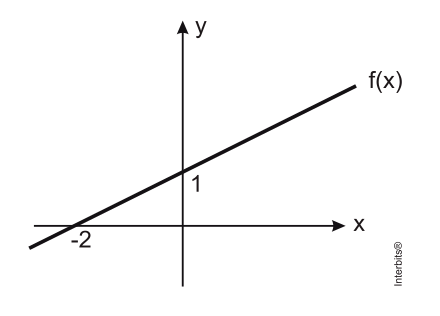
\includegraphics[width=\textwidth]{q06fig.png}
                    \end{figure}
                \end{column}
                \begin{column}{.4\textwidth}
                    A expressão algébrica que define a função inversa de $f(x)$ é:

                    \vspace{0.2cm}

            \begin{enumerate}
                \item $\displaystyle y = \frac{x}{2} + 1$ \vspace{2pt}
                \item $\displaystyle y = x + \frac{1}{2}$ \vspace{6pt}
                \item $\displaystyle y = 2x - 2$ \vspace{2pt}
                \item $\displaystyle y = -2x + 2$ \vspace{2pt}
                \item $\displaystyle y = 2x+2$
            \end{enumerate}
                \end{column}
            \end{columns}
        \end{enumerate}
            \end{column}
        \end{columns}
    \end{frame}
\end{document}